In this chapter we first lay out the results obtained in the experiments across
all 3 hypotheses, including some quick takeaways from the results. We then
compare the results across all experiments and explore some deeper discussion
points. We conclude the chapter by talking about future work and extensions to
the current methodology.

\section{Hypothesis 1}

Hypothesis 1 (H1) is stated as follows:

\begin{quote}
Explore some of the hyperparameters available during the feature extraction
process. The hypothesis is that using hyperparameter values more suited to
birdsong classification problems will yield a higher classification accuracy.
\end{quote}

H1 was applied to two feature extraction processes that appear in some form
widely in the literature related to birdsong classification: MFCC and GTCC\@.

\subsection{MFCC}

The key argument under test in this work as mentioned in
Section~\ref{sssec:mfcc} is the \texttt{BandEdges} argument. The results for the
AUC and classification accuracy for the 7 experiments listed in
Table~\ref{table:h1_mfcc_experiments} for MFCC can be seen in
Table~\ref{table:hyp1_mfcc} and can be visualized in Figure~\ref{fig:hyp1_mfcc}.

\begin{table}[ht]
\begin{center}
\begin{tabular}{cc c|c c}
\toprule
& \multicolumn{2}{c|}{AUC} & \multicolumn{2}{c}{Accuracy} \\
  Experiment & Linear & RBF & Linear & RBF \\ [0.5ex]
\midrule
  1 & \cellcolor{lightgray} 0.887 & \cellcolor{lightgray} 0.958 & 0.825 & 0.872 \\
  2 & 0.879 & 0.830 & \cellcolor{lightgray} 0.828 & 0.801 \\
  3 & 0.868 & 0.860 & 0.802 & 0.789 \\
  4 & 0.845 & 0.836 & 0.765 & 0.785 \\
  5 & 0.873 & 0.953 & 0.813 & \cellcolor{lightgray} 0.880 \\
  6 & 0.863 & 0.929 & 0.809 & 0.878 \\
  7 & 0.879 & 0.905 & 0.827 & 0.823 \\
\bottomrule
\end{tabular}
\caption{The AUC and classification accuracy scores for linear and RBF models
for different experiments for MFCC\@. The highest evaluation scores for each metric
and for each model are highlighted in grey.}\label{table:hyp1_mfcc}
\end{center}
\end{table}

\begin{figure}[ht]
  \centering
  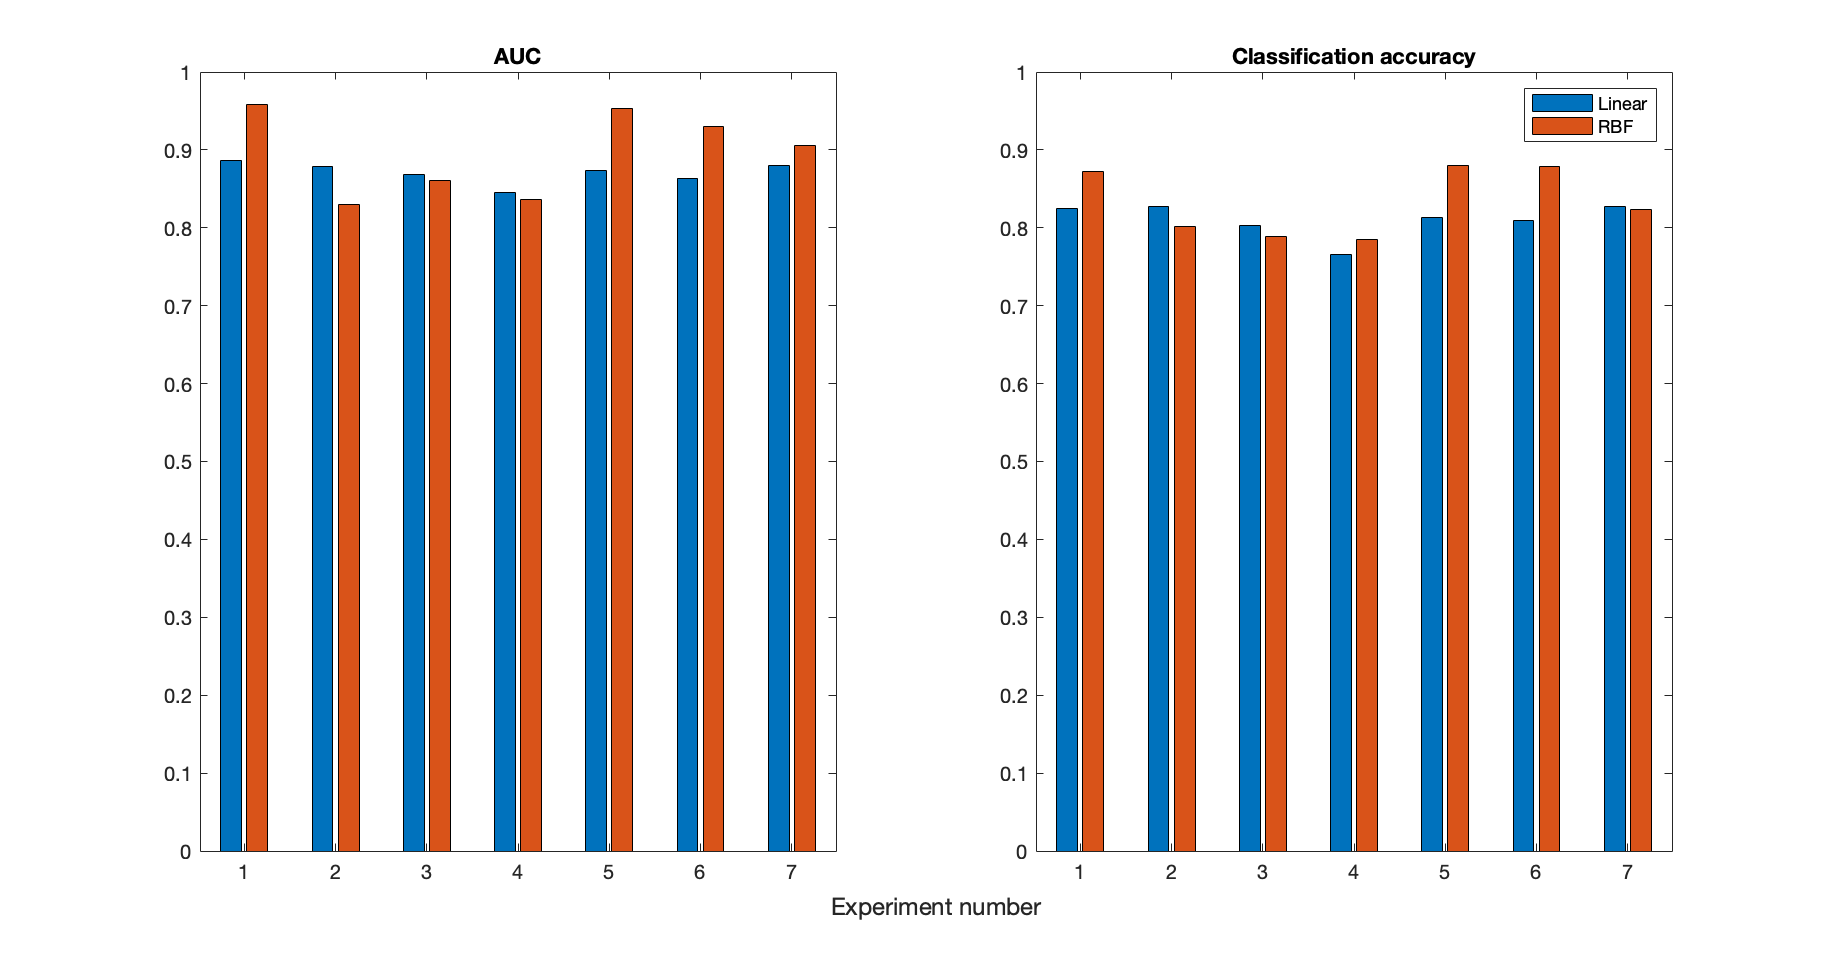
\includegraphics[width=\textwidth]{figures/hyp1_mfcc.png}
  \caption{The AUC and classification accuracy scores for linear and RBF models
  for different experiments for MFCC.}\label{fig:hyp1_mfcc}
\end{figure}

As shown in the table and chart, both evaluation metrics are around their
maximum in the control experiment (Experiment 1). Experiment 5 returns
comparable metrics to the control experiment, with slight improvements made to
the classification accuracy for the RBF model, but a slight reduction in the
AUC\@. The RBF model shows a clear reduction in performance for wider frequency
ranges across both evaluation metrics.

\subsection{GTCC}

The key argument under test in this work as mentioned in
Section~\ref{sssec:gtcc} is the \\ \texttt{FrequencyRange} argument. The results
for the AUC and classification accuracy for GTCC can be seen in
Table~\ref{table:hyp1_gtcc} and can be visualized in Figure~\ref{fig:hyp1_gtcc}.

\begin{table}[ht]
\begin{center}
\begin{tabular}{c c c|c c}
\toprule
& \multicolumn{2}{c|}{AUC} & \multicolumn{2}{c}{Accuracy} \\
  Experiment & Linear & RBF & Linear & RBF \\ [0.5ex]
\midrule
  1 & 0.884 & 0.895 & 0.844 & 0.802 \\
  2 & 0.887 & 0.946 & 0.831 & 0.856 \\
  3 & \cellcolor{lightgray} 0.891 & 0.933 & \cellcolor{lightgray} 0.852 & 0.850 \\
  4 & 0.883 & \cellcolor{lightgray} 0.948 & 0.846 & \cellcolor{lightgray} 0.859 \\
\bottomrule
\end{tabular}
\caption{The AUC and classification accuracy scores for linear and RBF models
for different experiments for GTCC\@. The highest evaluation scores for each metric
and for each model are highlighted in grey.}\label{table:hyp1_gtcc}
\end{center}
\end{table}

\begin{figure}[ht]
  \centering
  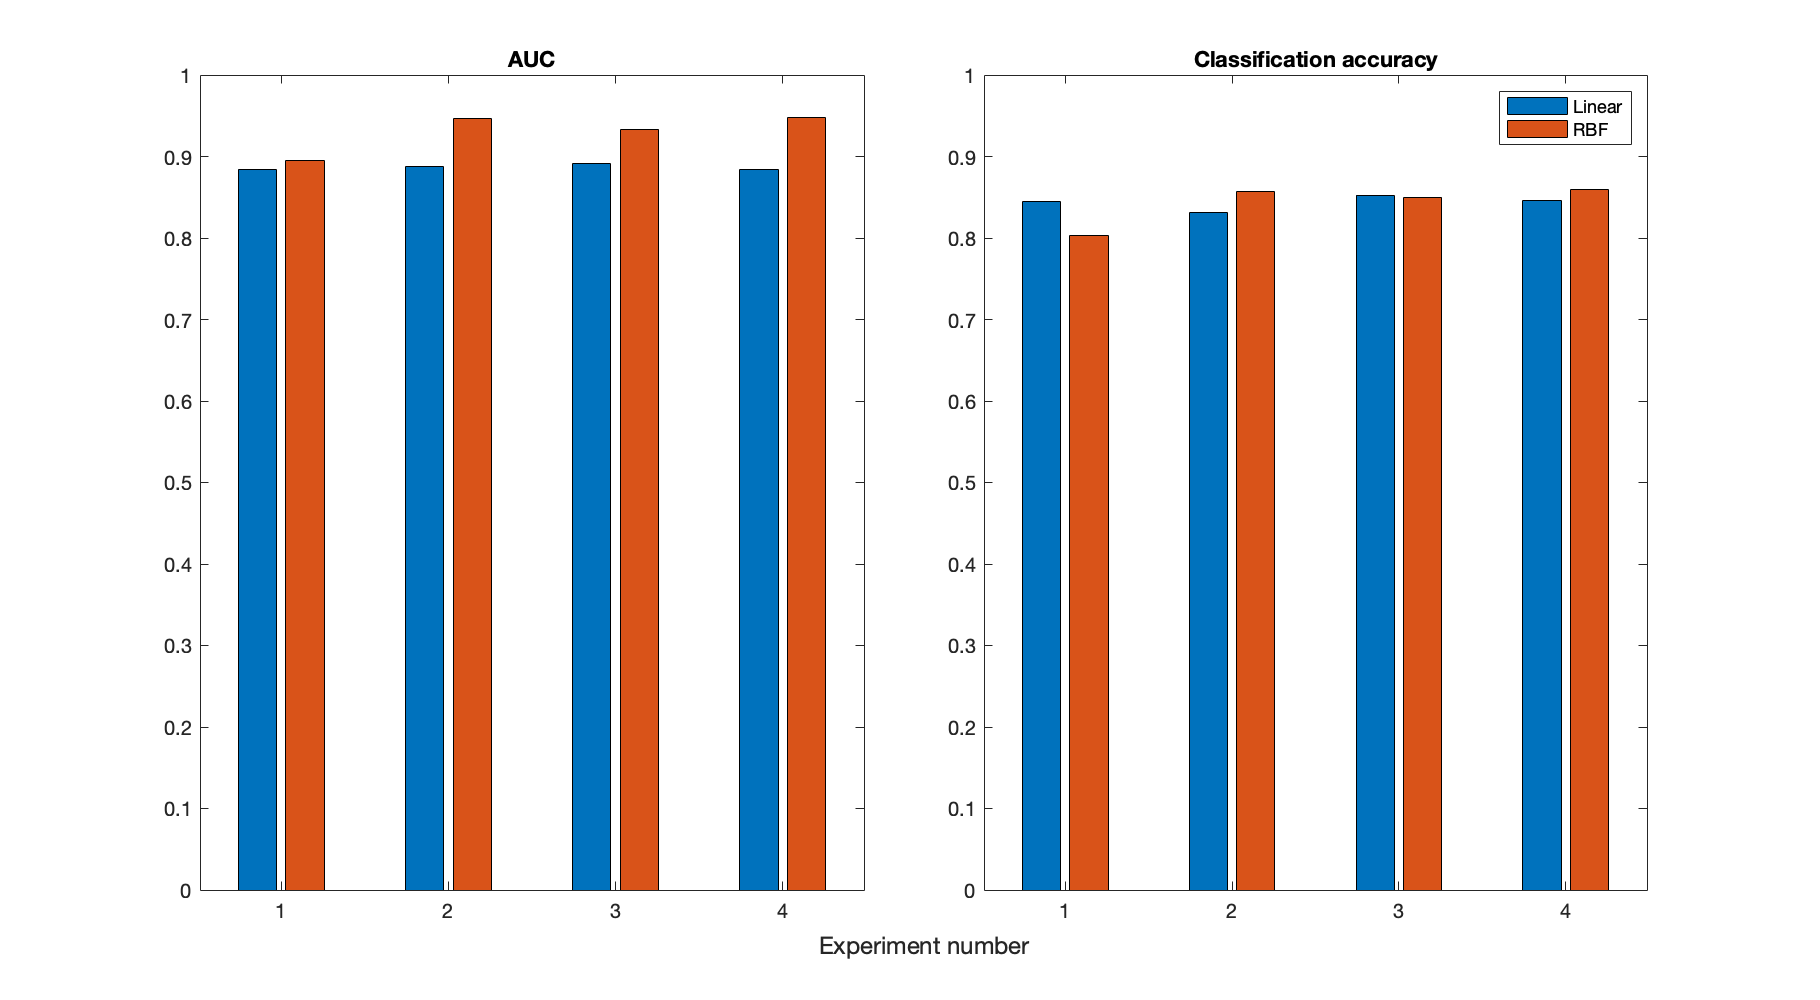
\includegraphics[width=\textwidth]{figures/hyp1_gtcc.png}
  \caption{The AUC and classification accuracy scores for linear and RBF models
  for different experiments for GTCC.}\label{fig:hyp1_gtcc}
\end{figure}

As shown in the table and chart, there is a significant increase in both metrics
for the RBF model when the frequency range is narrowed to be closer to the human
and birdsong vocalization range. The evaluation metrics for the linear model
remains largely similar across different frequency ranges.

\section{Hypothesis 2}

Hypothesis 2 (H2) is stated as follows:

\begin{quote}
Explore the performance of deep learning architectures such as Recurrent Neural
Networks (RNN) and Convolutional Neural Networks (CNN) and compare the results
with simpler statistical models. The hypothesis is that more complex and
flexible architectures such as these will have superior performance when
compared to simpler statistical models, such as SVMs.
\end{quote}

For all experiments related to H2 we use the highest performing feature
representations from H1: an MFCC representation with the \texttt{BandEdges}
argument set to the range from Experiment 1 and GTCC representation with the
\texttt{FrequencyRange} set to the range from Experiment 4.

\subsection{CNN}

The CNN architectures listed in Table~\ref{table:cnn_architectures} were tested
and their performance evaluated. The following section details the results.

\subsubsection{Results}

The results for the AUC and classification accuracy for a CNN trained on a MFCC
and GTCC representation of training sequences can be seen in
Table~\ref{table:cnn_mfcc_results} and can be visualized in
Figure~\ref{fig:cnn_mfcc_results}.

\begin{table}[ht]
\begin{center}
\begin{tabular}{c c c|c c}
\toprule
& \multicolumn{2}{c|}{AUC} & \multicolumn{2}{c}{Accuracy} \\
  Model & MFCC & GTCC & MFCC & GTCC \\ [0.5ex]
\midrule
  0 & 0.976 & 0.976 & 0.912 & 0.900 \\
  1 & 0.971 & 0.952 & 0.865 & 0.882 \\
  2 & \cellcolor{lightgray} 0.988 & \cellcolor{lightgray} 0.984 & \cellcolor{lightgray} 0.929 & \cellcolor{lightgray} 0.928 \\
\bottomrule
\end{tabular}
\caption{The AUC and classification accuracy for different CNN architectures
trained on MFCC and GTCC feature representations. The highest evaluation scores
for each metric are highlighted in grey.}\label{table:cnn_mfcc_results}
\end{center}
\end{table}

\begin{figure}[ht]
  \centering
  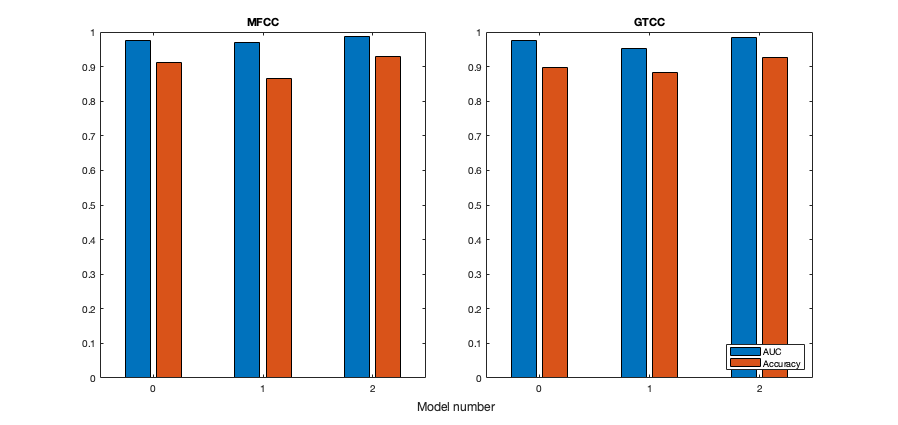
\includegraphics[width=\textwidth]{figures/hyp2_cnn_bar.png}
  \caption{The AUC and classification accuracy for different CNN architectures
  trained on MFCC and GTCC feature representations.}\label{fig:cnn_mfcc_results}
\end{figure}

We can see that the CNN models all deliver very promising results, especially
models 0 and 2. The highest performing of the CNN models is model 2, but it
should be noted that it takes significantly longer to train model 2 compared to
model 0 and its evaluation metrics are only slightly better.

\subsection{RNN \& CRNN}

The RNN and CRNN architectures listed in Table~\ref{table:rnn_seq_vector} were
tested and their performance evaluated. The following section details the
results.

\subsubsection{Results}

The results for the AUC and classification accuracy for a RNN and CRNN trained
on a MFCC representation of training sequences can be seen in
Table~\ref{table:rnn_mfcc_results} and can be visualized in
Figure~\ref{fig:rnn_mfcc_results}.

\begin{table}[ht]
\begin{center}
\begin{tabular}{c c c}
\toprule
Model & AUC & Accuracy \\ [0.5ex]
\midrule
1 & \cellcolor{lightgray} 0.957 & \cellcolor{lightgray} 0.892 \\
2 & 0.912 & 0.860 \\
3 & 0.887 & 0.840 \\
\bottomrule
\end{tabular}
\caption{The AUC and classification accuracy for different RNN and CRNN
architectures trained on MFCC\@. The highest evaluation scores for each metric
and are highlighted in grey.}\label{table:rnn_mfcc_results}
\end{center}
\end{table}

\begin{figure}[ht]
  \centering
  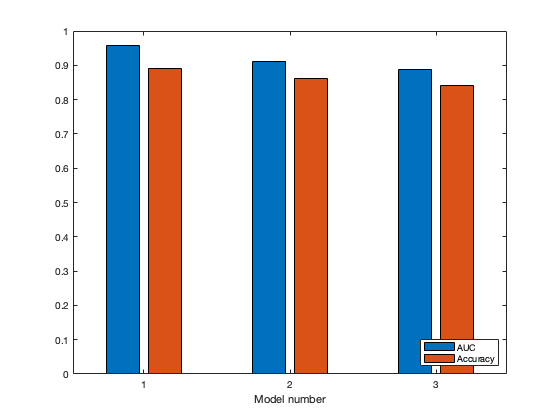
\includegraphics[width=0.8\textwidth]{figures/hyp2_rnn_mfcc_results.png}
  \caption{The AUC and classification accuracy for different RNN and CRNN architectures
  trained on MFCC.}\label{fig:rnn_mfcc_results}
\end{figure}

From the results we can see that model 1 performs the best across both metrics.
It should be noted though that model 1 takes the longest to train, about 5 times
longer per epoch compared to models 2 and 3. We can also see a clear drop in
performance comparing model 3 (a GRU model) to model 2 (a bidirectional LSTM
model). This is may be from the fact that the GRU layer cannot learn in both
directions, or it may be that the decrease in parameters that the GRU offers
comes at a cost of limited capacity to learn.

\section{Hypothesis 3}

Hypothesis 3 (H3) is stated as follows:

\begin{quote}
Explore the birdsong classification performance of feature representations
\\shown to have promising results for non-birdsong related audio classification
problems. The hypothesis is that feature representations shown to have good
results in audio classification problems will have good results for birdsong
identification.
\end{quote}

H3 was applied to a relatively novel feature representation, the MRCG, using
CNN, RNN and CRNN\@. To the author's knowledge, this experiment has not been
performed before with regards to birdsong classification.

Based on the results from the GTCC experiments shown in
Table~\ref{table:h1_gtcc_experiments}, we can see that a gammatone frequency
bank range of about 50 --- 10000 Hz works well for this problem. This range is
used in calculating the MRCG representation for all experiments.

Due to the high dimensionality of the MRCG representation and considering the
limited computational resources of the machine upon which training is performed,
we select simple NN models to evaluate the MRCG feature. The models chosen here
are Model 0 from Table~\ref{table:cnn_architectures}, and Models 1 and 2 from
Table~\ref{table:rnn_seq_vector}.

\subsubsection{Results}

The AUC and accuracy results for NN models trained on MRCG representation are
shown in Table~\ref{table:rnn_mrcg_results}.

\begin{table}[ht]
\begin{center}
\begin{tabular}{c c c}
\toprule
Model & AUC & Accuracy \\ [0.5ex]
\midrule
1 & \cellcolor{lightgray} 0.968 & \cellcolor{lightgray} 0.889 \\
2 & 0.188 & 0.283 \\
3 & 0.138 & 0.205 \\
\bottomrule
\end{tabular}
\caption{The AUC and classification accuracy for different RNN and CRNN
architectures trained on MFCC\@. The highest evaluation scores for each metric
and are highlighted in grey.}\label{table:rnn_mrcg_results}
\end{center}
\end{table}

The CNN model performs well but the RNN based models perform very poorly. The
training curve for the RNN models was still converging by the time that the
maximum number of epochs (100) was reached so it's possible that the model may
just need a longer time to train. However, during training the validation curve
fluctuated around 50\% and so it's also possible that the sequential vector
representation is inappropriate for an MRCG and so RNN with this type of
sequence input for MRCG will never post good results. Since the CNN results are
much better, it may be worthwhile exploring more complicated CNN model
architectures with MRCG\@. Due to the high dimensionality of MRCG I was not able
to perform training with more complicated models on my machine.

\section{Comparison}

In this section we collect the results from all experiments and compare them to
get a snapshot of the highest performing models. This may help to identify
patterns or trends in model structure or feature representation which boost
birdsong binary classification performance.

We start by listing all models used in this work. The SVM models used in this
work are listed in Table~\ref{table:svm_models} and the NN models are listed in
Table~\ref{table:nn_models}.

\begin{table}
\begin{center}
\begin{tabular}{c c c}
\toprule
Model ID & Feature & Description \\ [0.5ex]
\midrule
SVM\_M\_L\_1 & MFCC & Linear SVM with 40 mel bands, default range \\
SVM\_M\_R\_1 & MFCC & As above, but RBF SVM \\
SVM\_M\_L\_2 & MFCC & Linear SVM with 40 mel bands, extended range \\
SVM\_M\_R\_2 & MFCC & As above, but RBF SVM \\
SVM\_M\_L\_3 & MFCC & Linear SVM with 80 mel bands, extended range \\
SVM\_M\_R\_3 & MFCC & As above, but RBF SVM \\
SVM\_M\_L\_4 & MFCC & Linear SVM with 40 linear bands, extended range \\
SVM\_M\_R\_4 & MFCC & As above, but RBF SVM \\
SVM\_M\_L\_5 & MFCC & Linear SVM with 40 linear bands, default range \\
SVM\_M\_R\_5 & MFCC & As above, but RBF SVM \\
SVM\_M\_L\_6 & MFCC & Linear SVM with 40 anti-mel bands, default range \\
SVM\_M\_R\_6 & MFCC & As above, but RBF SVM \\
SVM\_M\_L\_7 & MFCC & Linear SVM with 40 mel bands, slightly extended range \\
SVM\_M\_R\_7 & MFCC & As above, but RBF SVM \\
SVM\_G\_L\_1 & GTCC & Linear SVM with default (widest) gammatone range \\
SVM\_G\_R\_1 & GTCC & As above, but RBF SVM \\
SVM\_G\_L\_2 & GTCC & Linear SVM with narrowed gammatone range \\
SVM\_G\_R\_2 & GTCC & As above, but RBF SVM \\
SVM\_G\_L\_3 & GTCC & Linear SVM with less narrow gammatone range \\
SVM\_G\_R\_3 & GTCC & As above, but RBF SVM \\
SVM\_G\_L\_4 & GTCC & Linear SVM with more narrow gammatone range \\
SVM\_G\_R\_4 & GTCC & As above, but RBF SVM \\
\bottomrule
\end{tabular}
\caption{Table listing the different SVM models used in this work. More details
for the MFCC models can be seen in Table~\ref{table:h1_mfcc_experiments} and
Table~\ref{table:h1_gtcc_experiments} for GTCC models.}\label{table:svm_models}
\end{center}
\end{table}

\begin{sidewaystable}
\begin{center}
\begin{tabular}{c c l c c}
\toprule
Model ID & Feature & Description & \# Learnable parameters & Training time/epoch (s) \\ [0.5ex]
\midrule
CNN\_M\_1 & MFCC & Simple 2 layer CNN & 32.5k & 3 \\
CNN\_G\_1 & GTCC & As above & 32.5k & 3 \\
CNN\_M\_2 & MFCC & 6 layer CNN based on~\cite{ruff2020automated} & 3.3m & 60 \\
CNN\_G\_2 & GTCC & As above & 3.3m & 60 \\
CNN\_M\_3 & MFCC & 8 layer CNN based on~\cite{kahl2017large} & 23.6m & 165 \\
CNN\_G\_3 & GTCC & As above & 23.6m & 165 \\
RNN\_M\_1 & MFCC & Simple 2 layer RNN & 112.4k & 16 \\
CRNN\_M\_1 & MFCC & 4 layer CRNN with BiLSTM layer & 142.5k & 3 \\
CRNN\_M\_2 & MFCC & 4 layer CRNN with GRU layer & 59.8k & 3 \\
CNN\_C\_1 & MRCG & Simple 2 layer CNN & 795.1k & 3 \\
RNN\_C\_1 & MRCG & Simple 2 layer RNN & 695.6k & 30 \\
CRNN\_C\_1 & MRCG & 4 layer CRNN with BiLSTM layer & 212.5k & 9 \\
\bottomrule
\end{tabular}
\caption{Table listing the different NN models used in this work. More details
for the CNN models can be seen in Table~\ref{table:cnn_architectures} and
Table~\ref{table:rnn_seq_vector} for RNN and CRNN models.}\label{table:nn_models}
\end{center}
\end{sidewaystable}

A combined table of evaluation metrics can be seen in
Table~\ref{table:all_results} and visualized in Figure~\ref{fig:all_bar}.

\begin{table}[ht]
\begin{center}
\begin{tabular}{c c c|c c c}
\toprule
Model ID & AUC & Accuracy & Model ID & AUC & Accuracy \\ [0.5ex]
\midrule
SVM\_M\_L\_1 & 0.887 & 0.825 & SVM\_G\_R\_2 & 0.946 & 0.856 \\
SVM\_M\_R\_1 & 0.958 & 0.872 & SVM\_G\_L\_3 & 0.891 & 0.852 \\
SVM\_M\_L\_2 & 0.879 & 0.828 & SVM\_G\_R\_3 & 0.933 & 0.850 \\
SVM\_M\_R\_2 & 0.830 & 0.801 & SVM\_G\_L\_4 & 0.883 & 0.846 \\
SVM\_M\_L\_3 & 0.868 & 0.802 & SVM\_G\_R\_4 & 0.948 & 0.859 \\
SVM\_M\_R\_3 & 0.860 & 0.789 & CNN\_M\_1 & 0.976 & 0.912 \\
SVM\_M\_L\_4 & 0.845 & 0.765 & CNN\_G\_1 & 0.976 & 0.900 \\
SVM\_M\_R\_4 & 0.836 & 0.785 & CNN\_M\_2 & 0.971 & 0.865 \\
SVM\_M\_L\_5 & 0.873 & 0.813 & CNN\_G\_2 & 0.952 & 0.882 \\
SVM\_M\_R\_5 & 0.953 & 0.880 & CNN\_M\_3 & \cellcolor{lightgray} 0.988 & \cellcolor{lightgray} 0.929 \\
SVM\_M\_L\_6 & 0.863 & 0.809 & CNN\_G\_3 & 0.984 & 0.928 \\
SVM\_M\_R\_6 & 0.929 & 0.878 & RNN\_M\_1 & 0.957 & 0.892 \\
SVM\_M\_L\_7 & 0.879 & 0.827 & CRNN\_M\_1 & 0.912 & 0.860 \\
SVM\_M\_R\_7 & 0.905 & 0.823 & CRNN\_M\_2 & 0.887 & 0.840 \\
SVM\_G\_L\_1 & 0.884 & 0.844 & CNN\_C\_1 & 0.968 & 0.889 \\
SVM\_G\_R\_1 & 0.895 & 0.802 & RNN\_C\_1 & 0.188 & 0.283 \\
SVM\_G\_L\_2 & 0.887 & 0.831 & CRNN\_C\_1 & 0.138 & 0.205 \\
\bottomrule
\end{tabular}
\caption{The AUC and classification accuracy for all models. The highest
evaluation scores for each metric across all models are highlighted in
grey.}\label{table:all_results}
\end{center}
\end{table}

\begin{figure}[ht]
  \centering
  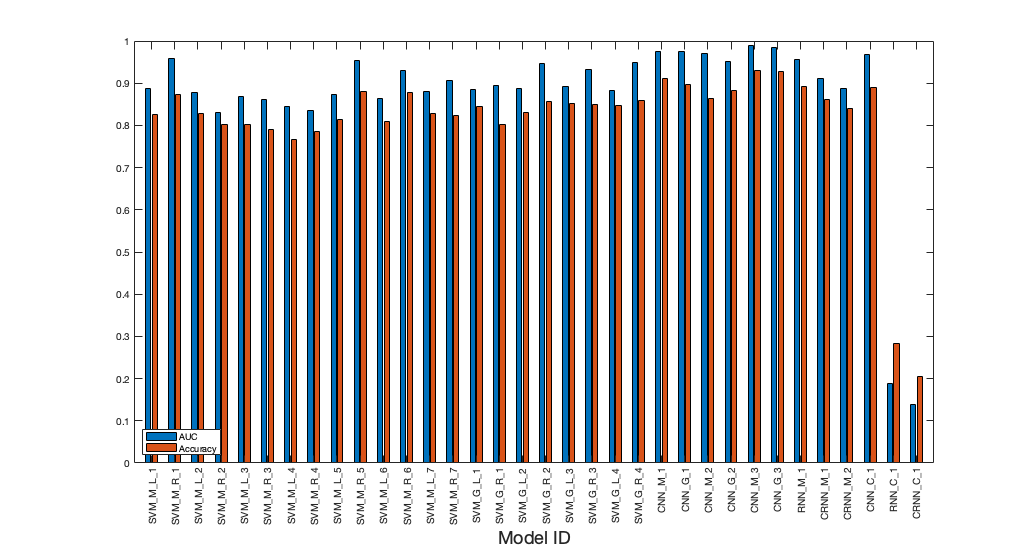
\includegraphics[width=\textwidth]{figures/all_bar.png}
  \caption{Figure showing the AUC and accuracy for all models tested in this
  thesis.}\label{fig:all_bar}
\end{figure}

\section{Discussion}

From the evaluation results obtained across the different experiments, the
following discussion points arise:

\begin{enumerate}

  \item A filterbank frequency range for feature representation that fits
    tightly around the dominant frequencies produced by birdsong performs better
    than one that is wider. This is strengthened by the results obtained from
    the experiments in H1. The initial assumption was that since birds produce
    higher frequency harmonics above the normal birdsong frequency range
    ($\backsim$1 kHz --- 10 kHz), then having a filterbank range that responds
    to those harmonics may mean that potentially useful features could be
    extracted from the harmonics and utilised by the model. In practice this
    doesn't seem to be the case, with both mel and gammatone filterbanks that
    range from $\backsim$1 kHz --- 10 kHz yielding the highest evaluation
    metrics. The assumption may have been naive since when comparing birdsong to
    human speech, as can be seen in Figure~\ref{fig:wren_vs_human}, we can see
    that both bird and human vocalizations produce strong harmonics. Given that
    MFCC with the default filterbank spacing has been shown to have excellent
    results with human speech recognition~\cite{muda2010voice}, it stands to
    reason that the default filter bank should have good results with birdsong
    too.

    \begin{figure}[ht]
      \centering
      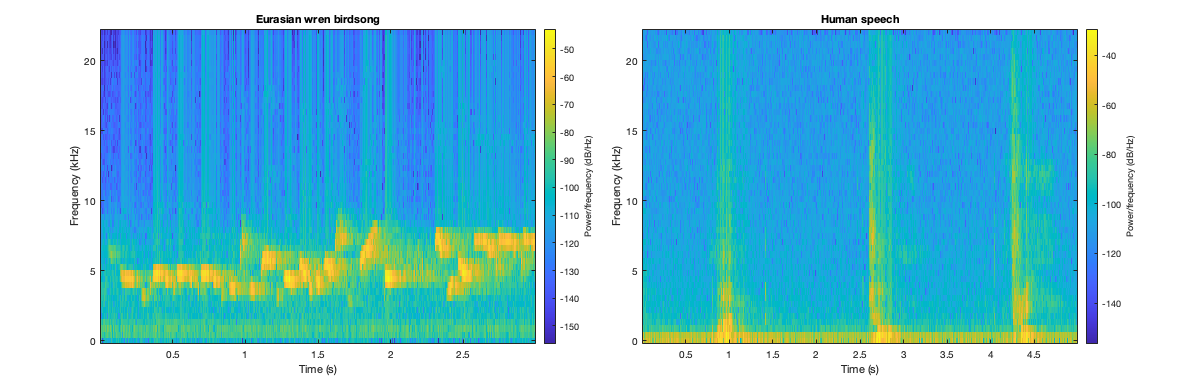
\includegraphics[width=\textwidth]{figures/wren_vs_human.png}
      \caption{Spectrograms of a sample from a Eurasian wren birdsong and human
      speech.}\label{fig:wren_vs_human}
    \end{figure}

    The other assumption with regards to filter bank range and spacing is that,
    since birdsong typically resides at higher frequencies than human speech (as
    can been seen in Figure~\ref{fig:wren_vs_human}), filter banks that are
    spaced closer together at higher frequencies (such as anti-mel filter
    banks), should offer more discriminatory power at higher frequencies and
    thus yield better results at discriminating birdsong. However, the results
    from the experiments performed in this work did not reinforce this claim and
    it remains unclear why.

  \item NN models can offer significantly improved metrics when compared to
    simpler statistical models such as SVM\@. Even the lowest performing NN
    model in this work (CRNN\_M\_2) trained on MFCC or GTCC posts metrics that
    are superior to the majority of SVM models tested here. This is reasonably
    unsurprising since NN models have considerably more learnable parameters and
    are able to fit more complex decision boundaries. This of course comes at a
    cost of higher computational demands and training time. While the RNN and
    CRNN model results are encouraging, it's important to note though that the
    models implemented here are quite simplistic. With some thorough tuning and
    testing I'm confident that the RNN models, in particular CRNN models, can
    achieve better evaluation metrics than plain CNN models. RNN models offer
    the enticing prospect of making use of the temporal evolution of birdsong
    and even learning from the gaps in between phrases, which may offer further
    information which can aid with classification.

  \item MRCG feature representations tested in this work have not performed as
    well as expected. This is disappointing since the literature has shown
    promising results when MRCG was used as a feature in audio classification
    problems. One thing to note though is that the literature has often tested
    MRCG at different SNR levels to determine its performance at classifying
    audio in noisy situations, where it has often outperformed more traditional
    feature representations~\cite{binti2020comparison,chen2014feature}. The
    samples tested in this work have all been very clean samples with little or
    no background noise, so it's possible that MRCG could start to become more
    effective when different SNR levels are tested with birdsong
    classification.

\end{enumerate}

\section{Further work \& extensions of methodology}

The work carried out in this thesis is merely scratching the surface of birdsong
binary classification problems. There is enormous scope for extending the
methodologies used here in pre-processing, training and classification in order
to improve results and broaden the problem. The following list is certainly not
exhaustive but is intended to provide a quick overview of some key techniques
and concepts that could be incorporated in future work.

\subsubsection{Pre-processing}

Pre-processing is a key stage in the process. A thorough and considered
pre-processing pipeline can significantly improve classification accuracy and
generalization performance. An easily accessible way to improve generalization
is through data augmentation. This has been done in many research papers with
promising results~\cite{kahl2017large}. \textit{MATLAB} provides inbuilt ways to
augment audio data through the \texttt{audioDataAugmenter} pipeline, which can
enlarge datasets through techniques like pitch shifting, time-scale
modification, and volume control. It would be interesting to apply these
augmentations and see how it affects the performance of these models. The
pipeline also offers noise addition. In practice, working with clean recordings
of birdsong would be very unlikely since the recordings would likely be
corrupted with all manner of background noise, from urban noise, rainforest
noise, or ambient noise such as wind, and so adding random noise through the
pipeline would certainly be useful. It might also be informative to manually add
noise at precise SNR levels and evaluate the performance of the different
feature representations and models in this work.

Another interesting extension of the methodology would be to consider a birdsong
segment as a variable length sequence of images as mentioned in
Section~\ref{sssec:method:rnn} where each syllable is transformed to some image
representation. This would allow for a system whereby syllables extracted from
birdsong could be fed into a RNN or CRNN with 2D convolutions. This could then
be used for realtime classification of birdsong, as is done in the excellent
Merlin\footnote{\url{https://merlin.allaboutbirds.org/}} app developed by
Cornell University Lab of Ornithology.

Lastly, a potential simplification of the pipeline could be to make more use of
the \texttt{detectSpeech} function. This is used in this work to strip leading
and trailing bits of background noise from recordings. With some experimentation
of the arguments it could potentially be used to perform the syllable
segmentation of the recording too.

\subsubsection{Feature extraction \& training}

An important concept missing in this thesis is combining features into stacks.
Instead of looking at feature representations in isolation, combinations of
features can be created and the model can be left to determine where the
important patterns lie in the dimensions of the data. This has been done in many
research papers~\cite{yan2021birdsong,ramashini2019bird,somervuo2006parametric}
to great effect. Chen et al.~\cite{chen2014feature} conducted thorough research
into a large number of feature representations in their work on speech
separation. This could be used as a basis for feature stacking extension to this
work.

The RNN and CRNN models implemented in this work are fairly naive and were
implemented to generate a baseline of the RNN method. With some experimenting of
the hyperparameters available, such as kernel size, pooling size and number of
convolutional layers, they could be shown to have improved performance.

\subsubsection{Classification}

Binary classification is a highly simplified version of the problem. In reality,
birdsong classification systems would likely need to classify birdsong into
hundreds or even thousands of classes. This could take the form of one sample
being assigned to one of many classes, or one sample which contains
vocalizations from different birds being able to accurately identify all the
classes contained therein. The former can be tackled using SVMs by turning the
problem into a one-versus-all classification, as mentioned in
Section~\ref{sssec:multiclass}. For NN models the modification is more simple.
The final dense layer can be modified to have the same number of output neurons
as classes and the softmax output layer will take care of outputting a
distribution over the classes. Identifying multiple birds within one sample
poses more challenges but there has already been some interesting research
conducted into it using encoder-decoder
architectures~\cite{narasimhan2017simultaneous}. Indeed, in their paper they
mention that future work includes adding recurrent layers to their network in
order to take into account the temporal relation between bird syllables.
